\section{Introduction} \label{sec:twins}
Since the microelectronics revolution, Silicon has been a dominant material for the production of devices for a variety of applications.
Silicon has non-ideal properties for a variety of applications but remains dominant due to its well-understood processing parameters and large manufacture install base, providing economies of scale.
The III-V semiconductors offer superior properties for a variety of applications when compared to silicon, and are actively used in applications were performance is valued above other considerations, such as military and space sectors.
The goal of integrating III-V semiconductors into silicon based microelectronics has spawned extensive research into the processing involved to grow or otherwise electronically attach these materials with minimal defects.

Under auspices of the ARISE Photovoltaics project, the III-V semiconductors GaAs, GaSb, AlSb and InP were grown as thin films under a variety of conditions on single crystal silicon substrates, to examine the growth process and electro-optic properties.
The role of the varied lattice mismatch, growth parameters, and substrate properties were examined and several previously undocumented phenomona were examined due to the use of 2DXRD, whose benefits were discussed in \cref{sec:2DXRD}.

The formation of epitaxial (or growth) twins was found to be a key area where the literature had performed little examination.
The role of twins in the formation of electronic defect networks, and the effects vicinal (offcut) substrates had on their formation were thoroughly examined and an explanatory model was developed to explain factors that affect their formation and provide proposed routes towards their minimization and elimination.
This work was published as ``The role of vicinal silicon surfaces in the formation of epitaxial
twins during the growth of III-V thin films'' in the Journal of Applied Physics\cite{Devenyi2011}
This work was completed in close collaboration with Ms.~Steffi Woo, now a Ph.D. candidate in Material Science and Engineering and McMaster, with the TEM/STEM work performed exclusively by her and all other work being collaborative.
\section{Background}
Anti-phase boundaries (APBs) have long been identified as highly detrimental to the electro-optic properties of epitaxial thin films\cite{Holt1969a}.
Extensive research has been performed in the use of vicinal substrates and other means\cite{Kroemer1987} to control the formation and propagation of APBs during the growth of epitaxial thin films.
A far more common planar defect during growth are epitaxial twins\cite{Ernst1989}.
Twins are regions of mirrored stacking sequence in the closest packed plane of \{111\} within a crystal with zincblende structure, where each consecutive layer is shifted after the first bounding stacking fault\cite{Wagner1966}.
These twin defects, often observed through transmission electron microscopy (TEM), have been attributed to a variety of causes, including APBs, threading dislocations and simple stacking faults\cite{Toyota2008b,Kim2006a,Xu2009,Proessdorf2010,Fischer1986a,Nguyen2004,Noge1987,Vila1995,Fischer1986}.
High resolution X-ray diffraction single peak analysis, which only examines X-ray peaks perpendicular to the substrate surface, will miss the additional peaks due to the presence of twins, leading to their misattribution.
Similarly, the sole use of conventional TEM has the disadvantage of being a local measurement, and not representative of the bulk.
Further work has definitively noted the key features of twins and provided guides to their identification\cite{Ernst1989}.

The twin has been considered a low-impact defect, due to its coherent interface and lack of dangling bonds, causing only weak scattering due to the minor disruption in the crystal symmetry.
This view of twins considers them as isolated in the material, ignoring the fact that in epitaxial films, twins are likely to intersect during growth, as the intersection of twins of different habit planes will lead to unsatisfied bonds.
For example, first-order twins formed on opposing habit planes can terminate from mutual intersection along a \{114\} plane, which is highly incoherent, resulting in unsatisfied bonds and trapped charge\cite{HORNSTRA1959}.
Furthermore, twins which intersect from adjacent habit planes will also form incoherent interfaces on high-order planes.
Finally, second- and higher-order twinning interfaces are expected to create dangling bonds, and will result in further unsatisfied bonds between the twinned regions and epitaxial film.

Using the combined techniques of two-dimensional X-ray Diffraction (2DXRD) and conventional TEM, this investigation has demonstrated a strong asymmetric suppression of twins due to the formation of atomic steps on vicinal substrates, previously observed for only GaAs\cite{Wei1994,Xie1990,Rajkumar1990}.
This combination of techniques allows macro and nano/micro characterization which combines to provide a complete analysis of a material system.
Twin suppression has been observed in GaAs, InP, GaSb and AlSb semiconductors grown on vicinal silicon substrates under varying growth conditions.
Through the integration of a quantitative reciprocal space mapping from 2DXRD and real-space imaging techniques from conventional TEM, we can understand the structural defects globally as well as their spatial distribution and propagation locally.
From this, we propose a comprehensive mechanism for the suppression, which is the asymmetric step-flow overgrowth of twins on vicinal substrates, applicable to all of the III-V material systems examined.
Given the detrimental nature of intersection of twins to electrical properties of thin films, this suppression phenomenon has the possibility of greatly improving the electro-optic properties of thin film III-V semiconductors grown on Si.
\section{Experimental}
Semiconductor epilayers (GaAs, InP, GaSb, and AlSb) were deposited on nominal (001)-oriented (\(\pm\)0.5\(^\circ\)) and vicinal Si substrates (offcut 4.7\degree{} (\(\pm\)0.25\degree) towards [110]) using a SVT Associates molecular beam epitaxy (MBE) system.
As-received epi-ready wafers were cleaned for 1~min in a 4\% HF in deionized (DI) water dip followed by a 30 sec DI rinse immediately before to their insertion into the MBE load-lock.
Before film deposition, both the nominal and vicinal Si(001) substrates underwent a 15~min degassing procedure at 350\celsius{} followed by a thermal treatment at 800\celsius{} for up to 5~min, to reconstruct the Si surface into single domain terraces\cite{NeergaardWaltenburg1995,S1991,Sakamoto1986,Pehlke1991}.
Few single steps are expected to remain on vicinal substrates, and a higher number on nominal substrates because of the larger terrace length.
Growth conditions followed established protocols\cite{Akahane2004,Balakrishnan2006a,Fischer1986} and yielded comparable rocking curve full-width half-maximum for the [004] reflection using HRXRD\@.
AlSb epilayers were grown to a thickness of 550~nm with a 20~nm GaSb capping layer to avoid oxidation.
GaAs epilayers was grown to a thickness of 600~nm and GaSb to a thickness of 500~nm.
InP samples were grown at 470\celsius{} with a V/III flux ratio of 2.0 at a growth rate of 1 \(\mu m\)/hr, resulting in a thickness of 600~nm.
HRXRD and TEM data also revealed that all films are fully relaxed by a network of interfacial misfit dislocations\cite{Vajargah2011}.
GaSb samples were grown in the presence of a 5~nm AlSb buffer layer, as prescribed by Akahane et al.\cite{Akahane2004}

Stereographic pole figures were generated for each sample using 2DXRD techniques.
A Bruker SMART 6000 CCD detector on a Bruker 3-circle D8 goniometer (Bruker AXS Inc., Madison, WI) with a Rigaku RU-200 rotating anode X-ray generator (Rigaku MSc, The Woodlands, TX) and parallel-focusing monochromator optics was used for the data collection.
Scans were taken with the detector centred on the (111) 2\(\theta\) of the material of interest and the sample rotated through 360\degree~in 0.5\degree~increments about the surface normal of the sample.
A 1D integration of all frames was used to determine the combined width of the (111) peaks using MAX3D software (McMaster University)\cite{Britten2007}.
The peak width was then used to integrate (111) reflections from all frames, including a background and absorption correction for the corresponding material with GADDS (Bruker-AXS) software, resulting in a pole figure.
Pole intensities were obtained from pole figures using a circular integration cursor with a 10 pixel radius which was centred on the pole such that the maximum total intensity was captured.
All pole intensities were corrected for structure factor and frame exposure times.

For each sample two \{110\} TEM cross-sections were prepared, one parallel to the [110] miscut direction and the other perpendicular.
The specimens were prepared by the standard procedure of mechanical polishing, dimpling, and ion-milling (4 keV Ar-ions at an incident angle of \(\pm\)4\degree~using a liquid nitrogen cold stage for InP) until perforation.
Crystallographic information of the epitaxial layer was obtained using diffraction contrast imaging with a Philips CM12 conventional transmission electron microscope (TEM) operated at 120 kV and equipped with a LaB\(_6\) filament.
In addition, electron diffraction analysis was performed using selected area electron diffraction (SAD).
\section{Results}
\cref{fig:twins_polefigure} shows the \{111\} pole figures generated from 2DXRD data.
The pole figures presented here are a stereographic projection of the (111) X-ray reflections of all orientations of the material of interest, oriented with the top of the figure corresponding to the [110] direction of the substrate.
The pole positions indicate that each of the III-V materials have the same symmetry and have variations of one orientation relationship with the Si substrate.
For each of the III-V films, the pole figures indicate a dominant [100]-orientation, as well as four weaker orientations associated with twins having (111), (1\(\overline{1}\)1)
(\(\overline{1}\overline{1}\)1)
and (\(\overline{1}\)11) habit planes, as indicated by a single shared pole (and hence a shared plane) between the bulk film and each twin variant.
A simulated pole figure, indicating the origin of each pole is labelled and given in \cref{fig:twins_sim_polefigure}.
The experimental pole figures differ from the simulation due to instrumental broadening of poles, and in that the AlSb and InP pole figures show second-order twinning, which is not included in the figure in an effort to maintain clarity.
The outermost poles are partially visible in the experimental pole figures due to limitations of the measurement range of samples in reflection, combined with substrate tilt tolerance.
The background of \cref{fig:twins_polefigure}(a) and (b) is higher due to the weaker X-ray scattering from GaAs.
For films grown on vicinal substrates (\cref{fig:twins_polefigure}(b),(d),(f),(h)) the centre of symmetry of the pole figure is shifted away from the tilt direction, i.e.\ towards the step edge.
\begin{figure}
 \centering 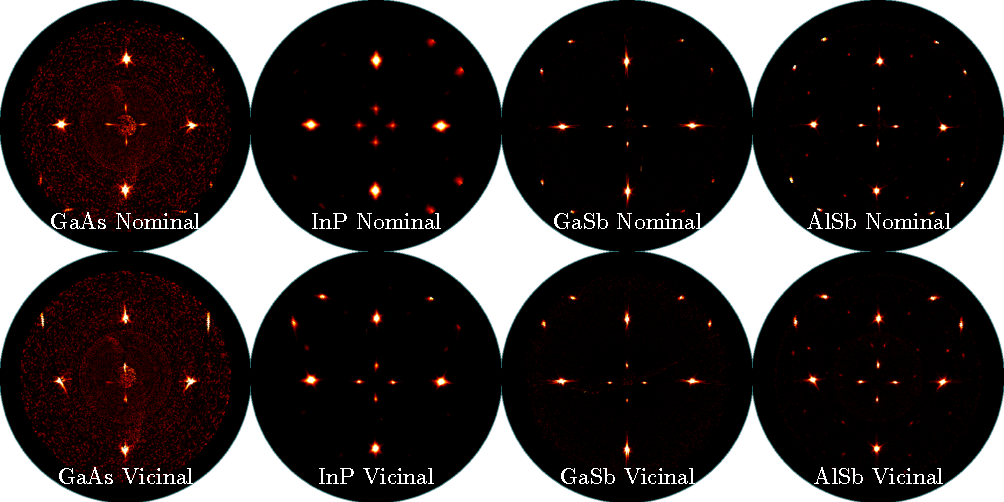
\includegraphics[width=0.9\textwidth]{twins_polefigure}
 \caption[Pole figures of nominal and vicinal substrates]{\label{fig:twins_polefigure}Stereographic \{111\} pole figures generated from 2DXRD show a bulk (100) phase plus four twinned variants as identified in \cref{fig:twins_sim_polefigure}.
  Twin variant intensity is asymmetric for vicinal substrates.}
\end{figure}
\cref{fig:twins_stats} shows the corrected measured and normalized intensity of the unique twin poles, as labelled in \cref{fig:twins_sim_polefigure}.
Measured intensities are normalized to the maximum value of pole intensity for each pole figure.
On nominal substrates, pole intensities are equal within experimental uncertainty and hence the twin volume fraction is equal for all four \(<\)111\(>\) twin plane directions.
Films grown on vicinal substrates, show a 50--75\% reduction in the volume fraction of the twin forming opposite to the step direction of the (111) habit plane (Pole 3).
The overall intensity of poles does not increase on vicinal substrates, as seen in the corrected intensity plot of \cref{fig:twins_stats}(a), indicating no overall increase in twinning due to vicinal substrates.
\begin{figure}
 \centering 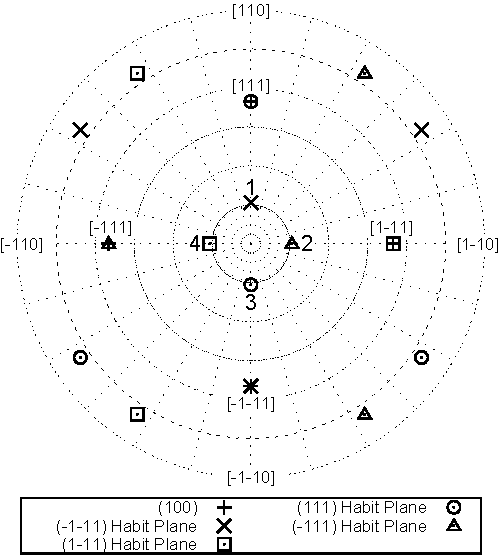
\includegraphics{twins_sim_polefigure}
 \caption[Simulated pole figure of twinned III-V on nominal silicon]{\label{fig:twins_sim_polefigure}Simulated \{111\} pole figure for a cubic III-V semiconductor film deposited on nominal silicon substrate.
  The pole figure containing poles from the dominant [100] film orientation film and from the 4 primary twins along their associated habit plane.
  The poles associated with each orientation are labelled with unique markers for use in the intensity measurements (\cref{fig:twins_stats}), and labels on the edge of the pole figure indicate absolute crystal directions of the silicon substrate.
  All poles from \cref{fig:twins_polefigure} are accounted for, although second-order twin poles are omitted for clarity.}
\end{figure}
Conventional cross-sectional TEM measurements indicate that microtwins are visible for all four of the III-V material systems studied.
Selected area electron diffraction (SAD) patterns of areas containing microtwins cause additional twin reflections in the form of streaks or spots in positions mirrored across the twin plane direction.
Analysis of the SAD patterns indicates that the twin variants in the GaAs epilayers are highlighted in strong contrast with dark-field (DF) images formed by isolating only the twin reflection of the dominant variant in the diffraction pattern (\cref{fig:twins_tem}(a) and (d)).
In comparison to their complementary DF images, where no particular twin variant is highlighted (\cref{fig:twins_tem}(b) and (e)), the preferential twinning direction is clearly present in GaAs grown on vicinal substrates.
This is also true for GaSb grown on vicinal substrates, as shown in \cref{fig:twins_tem}(f).
\begin{figure}
 \centering 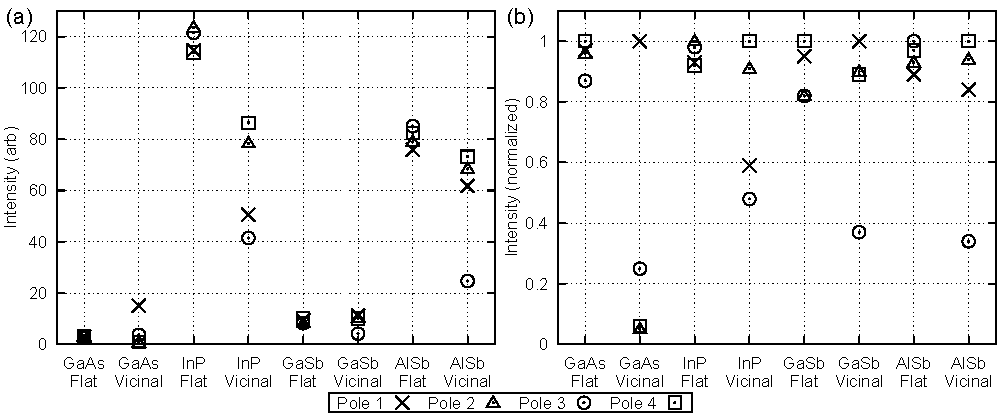
\includegraphics[width=\textwidth]{twins_stats}
 \caption[Integrated x-ray intensities from pole figures]{\label{fig:twins_stats}(a) Corrected (via structure factor and exposure time) and (b) normalized intensity of twin poles (as labelled in \cref{fig:twins_sim_polefigure} above).
  The normalized X-ray intensity shows a strong reduction in Pole 3 for all vicinal substrates.}
\end{figure}
The asymmetry in twinning directions for vicinal substrates is evident when examining their spatial distribution, as well as propagation into the epilayer with conventional TEM\@. The preferential twinning direction along
(\(\overline{1}\overline{1}\)1)
planes away from step edge (Pole 1) induces microtwins that propagate deep into much of the epilayer thickness, as indicated by microtwins with bright contrast in the DF image of GaSb and GaAs shown in \cref{fig:twins_tem}(f) and (d).
The intrinsic asymmetry to a vicinal substrate becomes obvious when viewing perpendicular to the tilt direction of [110].
The two edge-on \{111\} twin habit planes, namely
(\(\overline{1}\overline{1}\)1)
and (111) now lie 59.4\degree~(54.7\degree~\(+\) offcut angle) and 50\degree~(54.7\degree~\(-\) offcut angle) from the interface.
The reduction in peak intensity of Pole 3 from 2DXRD can now be explained by the TEM image of the representative variant, shown in \cref{fig:twins_tem2}, which propagates \(\sim\)25 nm from the interface and is small in width as visible in cross-section.
In addition, the in-situ RHEED pattern showed a transition from a spotty to a streaky pattern after nearly the same film thickness had been grown, indicating a change in surface morphology.
\begin{figure}
 \centering 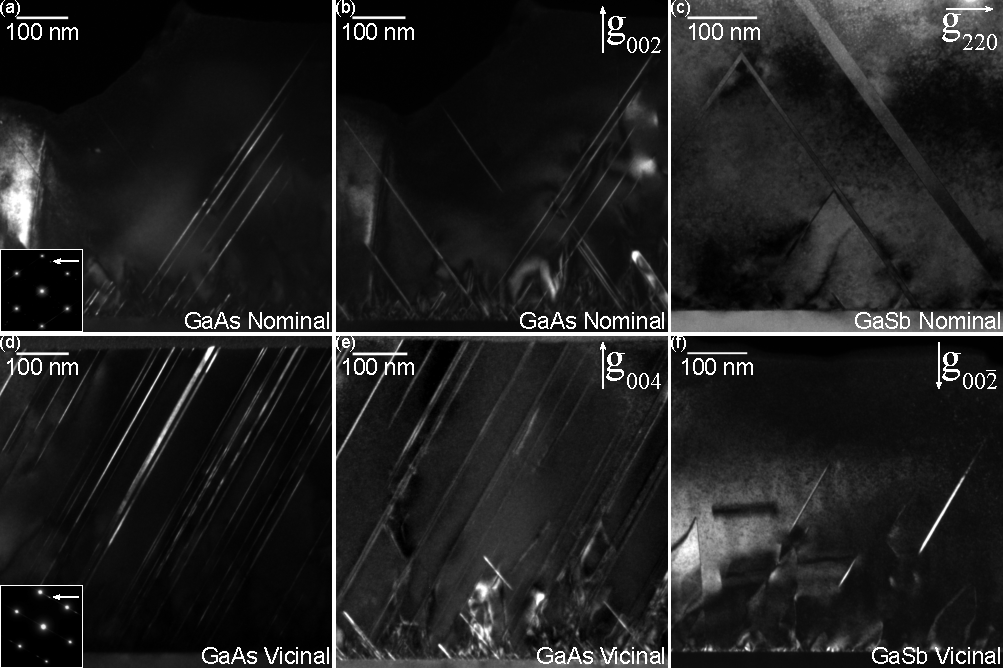
\includegraphics[width=\textwidth]{twins_tem}
 \caption[TEM images of III-V on silicon]{\label{fig:twins_tem}Conventional TEM images of the [1\(\overline{1}\)0] cross-section, (a) GaAs Nominal DF image of variants with
  (\(\overline{1}\overline{1}\)1)
  twin habit plane; (b) GaAs Nominal DF image of the same area as (a); (c) GaSb Nominal BF image; (d) GaAs Vicinal DF image of variants with
  (\(\overline{1}\overline{1}\)1)
  twin habit plane; (e) GaAs Vicinal DF image of the same area as (d); (f) GaSb Vicinal with the preferential twinning direction of
  (\(\overline{1}\overline{1}\)1)
  away from step edge (Pole 1), as indicated by microtwins with bright contrast in this DF image; step edge direction is towards the right for all vicinal images.}
\end{figure}
\begin{figure}
 \centering 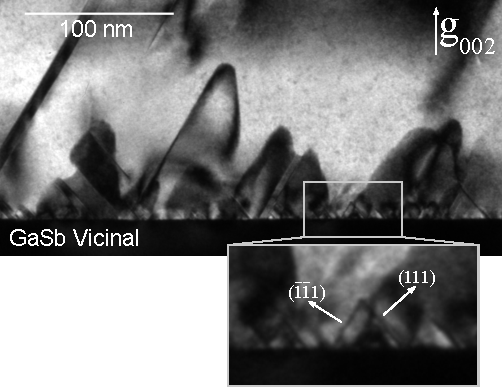
\includegraphics{twins_tem2}
 \caption[TEM of GaSb on silicon]{\label{fig:twins_tem2}Conventional TEM DF image of the [1\(\overline{1}\)0] cross-section of GaSb Vicinal, depicting the nanotwins close to the interface, of the twinning direction of (111) towards the step edges (Pole 3).
  The black ``n''-shaped loops in this DF image formed with a super-lattice reflection are APBs, as described by Woo et al.\cite{Woo}
  Step edge direction is towards the right of the image.}
\end{figure}
\section{Discussion}
Island nucleation followed by coalescence (i.e.\ the Volmer-Weber growth mode) is frequently observed for III-V thin films\cite{Ernst1989,Fang1990,Kim2010,Akahane2004}and is, in fact, anticipated for the growth parameters used in our film growths.
Both substrate strain and interfacial energy play a strong role in determining the size of the initial islands during nucleation.
After their initial formation, subsequent island growth occurs on the \{111\} planes, creating pyramidal structures which grow both laterally and in height.
For III-V systems, stacking along the \(<\)111\(>\) directions consists of alternating layers of group III- and group V-terminated surfaces, where two of the exposed surfaces are (111)A with Ga triply bonded, and the other two are (111)B with As triply bonded.
These two types of surfaces assemble at different rates.
Such a growth mode can continue indefinitely, but often transforms into a layer-by-layer growth once some critical thickness is achieved\cite{Tersoff1994}.
\begin{figure}
 \centering 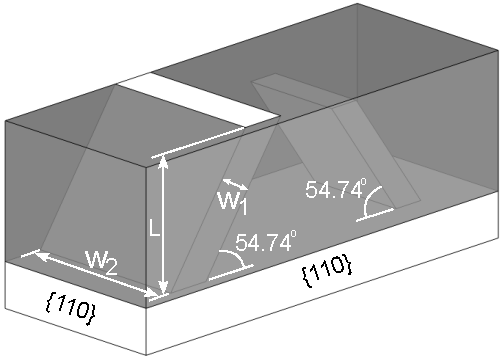
\includegraphics{twins_model}
 \caption[Model of twins on a (100) surface]{\label{fig:twins_model}Two twins on a nominal surface, embedded within a film.
  Twin dimensions with widths (\textit{w}\(_1\),\textit{w}\(_2\)) and length (\textit{L}) are labelled.}
\end{figure}
Epitaxial twins occur when atoms stacked on a \{111\} plane shift from their designated positions during growth, resulting in a stacking fault, characterized by a 180\degree{} rotation in bond directionality about the plane normal.
Atoms bonded to the next layer are likely to follow the stacking order defined by their nearest and next-nearest neighbour and continue the stacking sequence set out after the stacking fault, creating a rotation twin of the first region.
A subsequent stacking fault will then rotate the next layer back to its original orientation, bounding the twinned region.
The stacking fault energy (SFE) for a system is the measure of how costly it is for a single crystal plane to be misordered from its expected stacking sequence.

The total volume (V) of all twins in a film is given by \cref{eqn:twin_density} and schematically shown in \cref{fig:twins_model}:
\begin{equation}\label{eqn:twin_density}
 V \cong \sum\limits_{1}^{N} L w_1 w_2 \sin(54.74^{\circ})
\end{equation}
The first factor impacting the volume of twins in an epilayer is the number of twins (N).
This parameter is driven primarily by the SFE, but can also be influenced by the number of nucleation sites.
Atomic registration errors on \{111\} growth planes are expected to occur fairly frequently, as their probability is inversely proportional to the SFE, and SFE is only a fraction of the average thermal energy of an atom during growth\cite{Ernst1989}.
The formation energy of stacking faults is critical to the formation of microtwins, this is to say that when this energy is lower, the probability of a stacking fault, and hence twin formation, increases\cite{Oda2007}.
Higher assembly rates on the fault plane can also lock in stacking faults that could otherwise be corrected in order to minimize energetics.
The second factor, L, is the vertical length that the twins propagate through the epilayer, a value that generally is the full thickness of the epilayer.
The last two parameters impacting twin volume are the width in (w\textsubscript{1}) and perpendicular to (w\textsubscript{2}) the fast-growth direction.
The width of the twin in the growth direction is determined by the interplay between the SFE and the assembly rate of that plane.
The twin width perpendicular to the growth plane is determined by the size of the island in that dimension, which is influenced both by the chemistry and misfit of the epilayer-substrate interaction.

Given the role parameters play in twin volume fraction, it is now possible to account for the differences between the different III-V semiconductor films grown on nominal (001)-oriented Si substrates.
The most obvious difference is the mean volume of twins, with InP standing out as having the largest value.
This can mainly be attributed to the low value of 17 meV/atom for its reduced SFE (the energy per atom in a fault plane)\cite{Gottschalk1978}, as compared to the larger values of 47 and 53 meV/atom exhibited by GaAs and GaSb\cite{Gottschalk1978}.
It is noted that the SFE for AlSb has not been reported, but is expected to be similar to that of GaSb due its similar ionicity\cite{Holt2007b}.
The higher mean value exhibited by AlSb is due to its higher nucleation density\cite{Akahane2004}, which leads to a greater number of islands where each has the possibility of forming twins.

In all III-V films grown on vicinal substrates, there is a 50--75\% reduction in the volume of twins contributing to Pole 3.
This corresponds to a substantial reduction in twin formation opposite to the tilt direction.
GaAs, however, is unusual in that it exhibits a strong reduction in twins for directions perpendicular to the step direction (Pole 2 and 4), and an increase in twins towards the tilt direction (Pole 1 \(>>\) Pole 3).
The TEM studies of Xie et al.\cite{Xie1990} on GaAs epilayers grown on vicinal Si substrates observed with conventional TEM correlate well with our observations of As-initiated vicinal GaAs films.
Irrespective of the rotation in tilt direction to the perpendicular \(<\)110\(>\) between Xie's work and the work presented here, the same very low density and equal distribution of microtwins with \{111\} habit planes perpendicular to the tilt direction (Pole 2 and 4) is evident.
Xie's work proposed preferentially oriented island nucleation, and claimed that the asymmetric distribution of microtwinning is due to the two (111)B planes that are aligned with the offcut exhibiting a faster growth rate.
The reductions in the Pole 2 and 4 twin variants are not observed for the other III-V systems (i.e.,
InP, GaSb, and AlSb), indicating that the fastest-growing plane cannot be solely responsible for such reductions.
The single domain nucleation achieved by Xie due to Ga and As equal bonding preference to Si\cite{Bringans1988} cannot be guaranteed in other systems due to the lower bonding affinity of Sb\cite{Kubiak1985} and P\cite{Kiyota2001}.
These other systems instead show a behaviour in the distribution of microtwins that is a combination of the As-initiated and Ga-initiated GaAs, as demonstrated by Xie, indicating mixed domain nucleation (both group III and V atoms as first atomic layer species).
Despite the effort to use a group V-soaking before growth, the high affinity of group III atoms for Si can easily displace any weakly bonded group V atoms, especially at higher growth temperatures.
In growths of group III-initiated nucleation, the fastest growing planes remain as group V planes, but are rotated to the two perpendicular \{111\} orientations not under the influence of the substrate offcut asymmetry, as claimed by Xie.
Therefore, in the event of mixed domain nucleation, the asymmetric preferential growth of microtwins tilted towards the tilt direction in III-Vs grown on vicinal Si cannot be attributed exclusively to the faster growing group V planes.

Previous work by Wei and Aindow\cite{Wei1994} on GaAs epilayers on vicinal Si concludes that under a balanced Ga- and As-initiated flux, it is expected to achieve layer-by-layer growth.
They proposed that the high density of twins with habit planes towards the tilt direction in combination with less twins on all other habit planes is due to the deformation resulting from the residual misfit associated with the heteroepitaxy.
The critical resolved shear stress (i.e.\ the threshold value of stress necessary to cause atomic planes to slip) as calculated by Wei and Aindow\cite{Wei1994} along the \(<\)112\(>\) slip direction in the \{111\} planes towards the tilt direction is over 4\% higher than all other slip systems.
This means the likelihood of slip in this direction is lower, so deformation twins would more likely form.
This slip direction is not one of the two contributing partial dislocations (from the dissociation of a perfect dislocation along an interfacial \(<\)110\(>\) direction) responsible for the formation of a stacking fault common in such epilayers.
Therefore the twins observed cannot be exclusively or even primarily be due to deformation, as their asymmetric distribution cannot be explained by the anisotropy in resolved shear stresses alone.

Comparing nominal and vicinal samples for all systems, the vicinal substrates increase the mean intensity of twins, which can be attributed partially to an increased number of preferential nucleation sites during initial growth, thus increasing the number of twins (N), which can form.
Next, vicinal substrates enhance the fraction of twins with
(\(\overline{1}\overline{1}\)1)
habit planes oriented towards the tilt direction in GaAs, which is not observed for GaSb, AlSb and InP\@. This phenomenon is evident in both the 2DXRD intensity of Pole 1 (see \cref{fig:twins_stats}(a)) and the DF TEM image (see \cref{fig:twins_tem}(d)).
The work of Xie et al.
also shows that the As-initiated GaAs growth induces an exclusively As-prelayer which leads to a domain in which (111)B surfaces are on (111) and
(\(\overline{1}\overline{1}\)1)
aligned with the step direction.
The high assembly rates of those planes increase the probability of errors in the form of stacking faults, which, in turn, increases the total number of twins nucleated (N).
While in the case of mixed domain nucleation with GaSb, the enhancement in the
(\(\overline{1}\overline{1}\)1)
fast-assembly surface is diluted by the even distribution to the adjacent (1\(\overline{1}\)1) and (\(\overline{1}\)11) planes of equal assembly rates.
Because of this, fewer stacking errors occur in the
(\(\overline{1}\overline{1}\)1)
and (111) planes, and the number of twins nucleated along those planes are decreased.
The effects of this enhancement in the fraction of twins in III-Vs (including GaAs) is expected to be less pronounced with increasing growth temperature, where the group V-prelayer atoms are more likely to desorb, causing mixed nucleation and results which are more comparable to those of GaSb and AlSb.
The presence of single steps on vicinal substrates can also affect this enhancement phenomenon, as they cause a rotation of domains, which result in APBs.
The strong asymmetry in GaAs samples indicates that the Si substrate preparation results in mostly double-stepped vicinal substrates.

The sum of the four reflection intensities for GaSb grown on vicinal substrates is close to two times higher than for GaAs grown on vicinal substrates.
This is evident when comparing the width of twin domains with (111) and
(\(\overline{1}\overline{1}\)1)
habit planes in GaSb grown on nominal and vicinal Si substrates which are about two times as wide as those in GaAs, as shown in \cref{fig:twins_tem}(c) and (f), demonstrating an overall increase in the volume fraction of those twin variants.
The width of twins in GaSb grown on nominal and vicinal Si substrates with two (1\(\overline{1}\)1) and (\(\overline{1}\)11) habit planes are also about three times as wide as those in GaAs.

The proposed mechanism for the reduction of twins is the transition to a step-flow growth mode induced by vicinal substrates.
On nominal oriented substrates a transition to layer-by-layer growth allows for the continued propagation of nucleated epitaxial twins throughout the film as the growth front propagates normal to the substrate.
In some systems on nominal substrates, layer-by-layer growth is never achieved, as is observed for InP and AlSb.
On vicinal substrates, growth does not transition to a pure layer-by-layer growth mode but instead to a step-flow growth mode, due to the steps present on the underlying substrate.
From the transition point onwards, the growth front is not normal to the substrate, but instead flows across the surface at an enhanced rate towards the tilt direction.
This enhancement can also increase the fraction of twins forming in the step-flow direction as is the case for GaAs grown on vicinal substrates.
Growth fronts originating from the steps flow across the surface and overgrow islands that formed during the initial island growth mode.
Since step-flow growth occurs down steps, towards the tilt direction, twins which were initially nucleated on habit planes away from the tilt direction during island growth are halted since they need to propagate opposite to the growth front.
The transition from island to step-flow growth is evident due to the presence of nanotwins which propagate \(\sim\)25~nm from the interface before termination, as shown in the GaSb TEM DF image (\cref{fig:twins_tem2}).
This propagation distance into the film thickness is consistent with the transition from an island to step-flow growth mode as is apparent from the observed transition from a spotty to streaky RHEED pattern during the GaSb growth.
The transition to step-flow growth ultimately decreases the propagation length (L), of the twins with habit planes opposite to the tilt direction.

Greater vicinal angles are expected to initiate step-flow growth from nucleation, and hence eliminate twins opposite the tilt direction.
An offcut towards the [100] direction can induce surface steps in the two orthogonal \(<\)110\(>\) directions simultaneously\cite{Fang1990}, which is expected to decrease the twin density in two of four \{111\} habit planes, reducing the overall intersections of microtwins that do so along incoherent interfaces.
\section{Implications for Symmetry and Energy at Epitaxial Surfaces}
The growth of polar semiconductors, particularly the III-V on non-polar substrates such as silicon has presented significant challenges.
Besides the obvious issues regarding the intrinsic lattice mismatch between these epilayers and the proposed substrate, the uniform energy surface presented by a non-polar surface provides a poor template for the nucleation of polar semiconductors, introducing numerous electrically active defects.
Intentional symmetry breaking through the use of vicinal substrates provides a route to improve the quality of thin films, and to control the formation of defects.

By breaking the symmtery on the (100) silicon surface by the use of vicinal substrates, an important change to the energy landscape for a growing crystal, improving the overall quality of the film.
As has been documented numerous times in literature, vicinal substrates reconstruct at high temperatures in order to present the closest low energy (low index plane) surface, separated by atomic height steps.
When the offcut angle is sufficiently large, and the temperature processing sufficiently aggressive, the vicinal substrate reconstructs to present the same sublattice layer, separated by double height steps.
This uniform sublattice layer presents a chemical energy landscape for the incoming polar semiconductor atoms which results in the preferential nucleation of one of the two constituents, resulting a substantial or complete elimination of anti-phase boundaries.

The microtwinning observed in III-V compounds in literature had been ignored due to the assumption that twin interfaces are low-energy and non-defective.
The interaction of multiple twins on different habit planes however, has been demonstrated to present an incommensurate boundary between the two crystallites resulting in electrically active defective bonds.
By breaking the symmetry on the (100) silicon surface, growth twins, which frequently travel through the entire grown film, can be suppressed or limited to an interfacial region.
The introduction of the reconstructed vicinal surface presents step edges where adatoms are more likely to nucleate, overgrowing twins which spontaneously form during nucleation, confining the defects to a thin interface region.

While these results were not of immediate use to the ARISE project, due to the device of interest being a solar cell with vertical transport, horizontal transport devices grown epitaxially on silicon may benefit from the reduction in twin collisions forming in their active regions.
The twin suppression results here also point towards two future areas which may yield further improvements, larger offcut angles and different offcut directions.

Larger offcut values for vicinal substrates are known to increase the density of step edges to the point where the surface reconstructs to another low index plane.
Higher density steps are expected to increase the nucleation rate at edges, resulting in enhanced step flow, and further suppression of twinning.
Offcut directions other than [110], specifically 45\degree~between [110] and [211] will result in atomic reconstruction of the surface into two dimensional terraces with step edges along [110] and [211] directions.
Such two dimensional terraces could allow step flow growth and hence suppress twinning in two perpendicular directions, resulting in further reductions in twin collisions and reduction in defect density.
